\textbf{Cas d'utilisation:} Passer le péage
    
\textbf{Acteur primaire (initiateur):} Conducteur
    
%\textbf{Acteur support:} -

\textbf{Pré-condition: } Nécessite que la voie soit ouverte et libre

    
\textbf{Post-condition: }   La voie redevient disponible(ouverte et libre) pour un prochain usager.
    
\textbf{Scénario primaire: } \\
\textbf{1.} Le conducteur rentre dans la voie d’autoroute.(\ref{subsec:rentre})
 \\
\textbf{2.} Le conducteur paie le passage. (\ref{subsec:paie})\\
\textbf{3.} Le conducteur sort. (\ref{subsec:sortir})\\
    
\textbf{Variantes}\\
\textbf{1a.} Le conducteur n’arrive pas a rentrer dans la voie, dépannage et fin du scénario.\\
\textbf{3a.} le conducteur ne sort pas : la barrière reste fermer en attendant la sortie de conducteur.\\

\textbf{Décomposition des cas d'utilisation:} 
\begin{figure}[h]
    \centering
    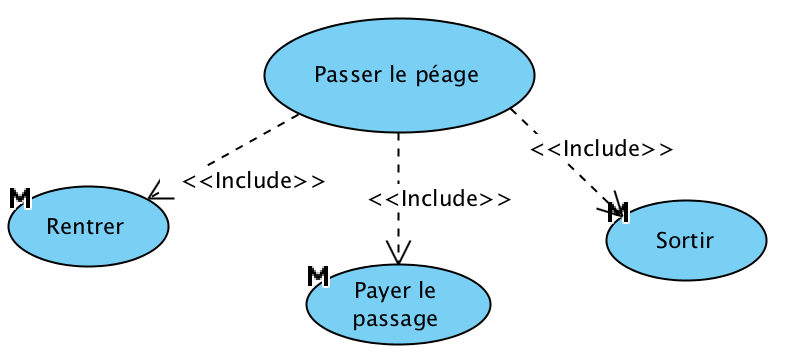
\includegraphics[scale=0.7]{02_Desenvolvimento/TD2/images/passerLePassage.png}
    \caption{Décomposition des cas d'utilisation: Passer le péage}
\end{figure}
